% Copyright James Percent 2013.
% All Rights Reserved.

\documentclass[11pt]{article}
\usepackage{graphics}
\usepackage{amsmath, amsthm, amssymb, latexsym}
\usepackage{hyperref}
\usepackage{draftwatermark}
\begin{document}

\title{\textbf{Unlock: A Framework for Programming Brain-Computer Interfaces}}
\author{James Percent \\
james@shift5.net}
\date{\today}
\parskip 11pt
\parindent 0pt
\maketitle
\tableofcontents
\section{Overview}\label{overviewsec}

Our goal is to develop BCI technology to help individuals suffering from locked-in syndrome (LIS)~\cite{lis} communicate.  LIS is characterized by an almost complete inability to communicate.  With current technology, unfortunately, we cannot achieve this goal.

We think, if more smart people are able to painlessly collaborate, then we have a better shot at accomplishing this goal.  Therefore, our [simple] strategy is to focus on providing an awesome programming framework that makes it easier for researchers and engineers to build BCI-based systems.  To this end, we employ a few simple ideas.  

We encapsulate as much as possible; this is kind of technical mumbo jumbo for trying to say that we separate concerns.  We'll talk more about this later, but the basic idea is that you should not need to know every corner of Unlock to create a new decoding algorithm or add a language model or add a new acquisition device or create a new application.  

These could be different people with different skill sets, and we want them to be able to dive into their area and be productive quickly.  One of the problems with BCI technology is that it is inherently cross-disciplinary; therefore, we want to lessen this burden as much as possible.

To support this goal, we need great documentation.  The documentation needs to be encapsulated too.  You should be able to get a high-level idea of how the whole system works and also locate details about your specific area of interest without arduous effort.  

Finally, automate whenever possible; extra batteries included.  We want researchers and engineers to be able to get going quickly.  Learning about all the dependencies and taking a bunch of manual steps can be overwhelming.  Especially if someone just wants to hack out a quick idea.  

In summary, the goal is to give you a great platform to hack out an idea.

The rest of this document is structured as follows.  %In the next section we provide a bit of history.
First we do a quick technical introduction.  After that, we discuss how to install and use Unlock, from a user perspective.  Next, we cover both some of the internals from a high-level.  Finally we close with a example.

Development of the Unlock framework is funded by the Adaptive Brain-Computer Interactions (ABCI) Capstone Project~\cite{abci}.

\section{Technical Introduction}

The infrastructure Unlock provides can be logically separated into two distinct layers: the application layer and the BCI layer.  These layers can in turn be further decomposed.

 The BCI layer is defined by the signal-processing chain~\cite{signalprocessing}.  The signal-processing chain includes signal acquisition and reconstruction, feature extraction and decoding, and command generation~\cite{neuraleng}.  Many BCI systems also include a stimulation component, which is actually processed at the application layer; however, logically, the stimulation component is part of the BCI.

For example, a paradigm based on Visually Evoked Potentials (VEP), flashes a graphical sequence at the user, which is subsequently interpreted in the signal-processing chain~\cite{vep}.  But the actual flashing is handled at the application layer.

We'll talk in more detail about the BCI layer in Section~\ref{bcisec}, but for now there is one important take away.  At each point in the pipeline we just discussed, the system is designed so that you can easily decorate, replace or otherwise manipulate the data flow.  Each step in the pipeline is encapsulated under an interface contract.

The application layer is model-view-controller (MVC)~\ref{mvc, mvc1} inspired.  Don't worry too much if you're not familar with MVC.  It's just a logical framework for structuring graphical user interfaces (GUIs).  

The basic idea is that each application consists of three types of objects: models, views and controllers.  The controllers accept user input (in this case BCI commands) and pass the inputs to the correct models.  Models handle state transformation (the business logic if you will).  Finally, views observe the state objects (models) and render themselves based on the current state of the world.

If you think about it, this also creates a pipeline in the application layer.  The take away here is that these components are also encapsulated under interfaces.

Figure~\ref{bci-pipeline-fig} depicts the data flow through Unlock.

\begin{figure}[]
\resizebox{\textwidth}{!}{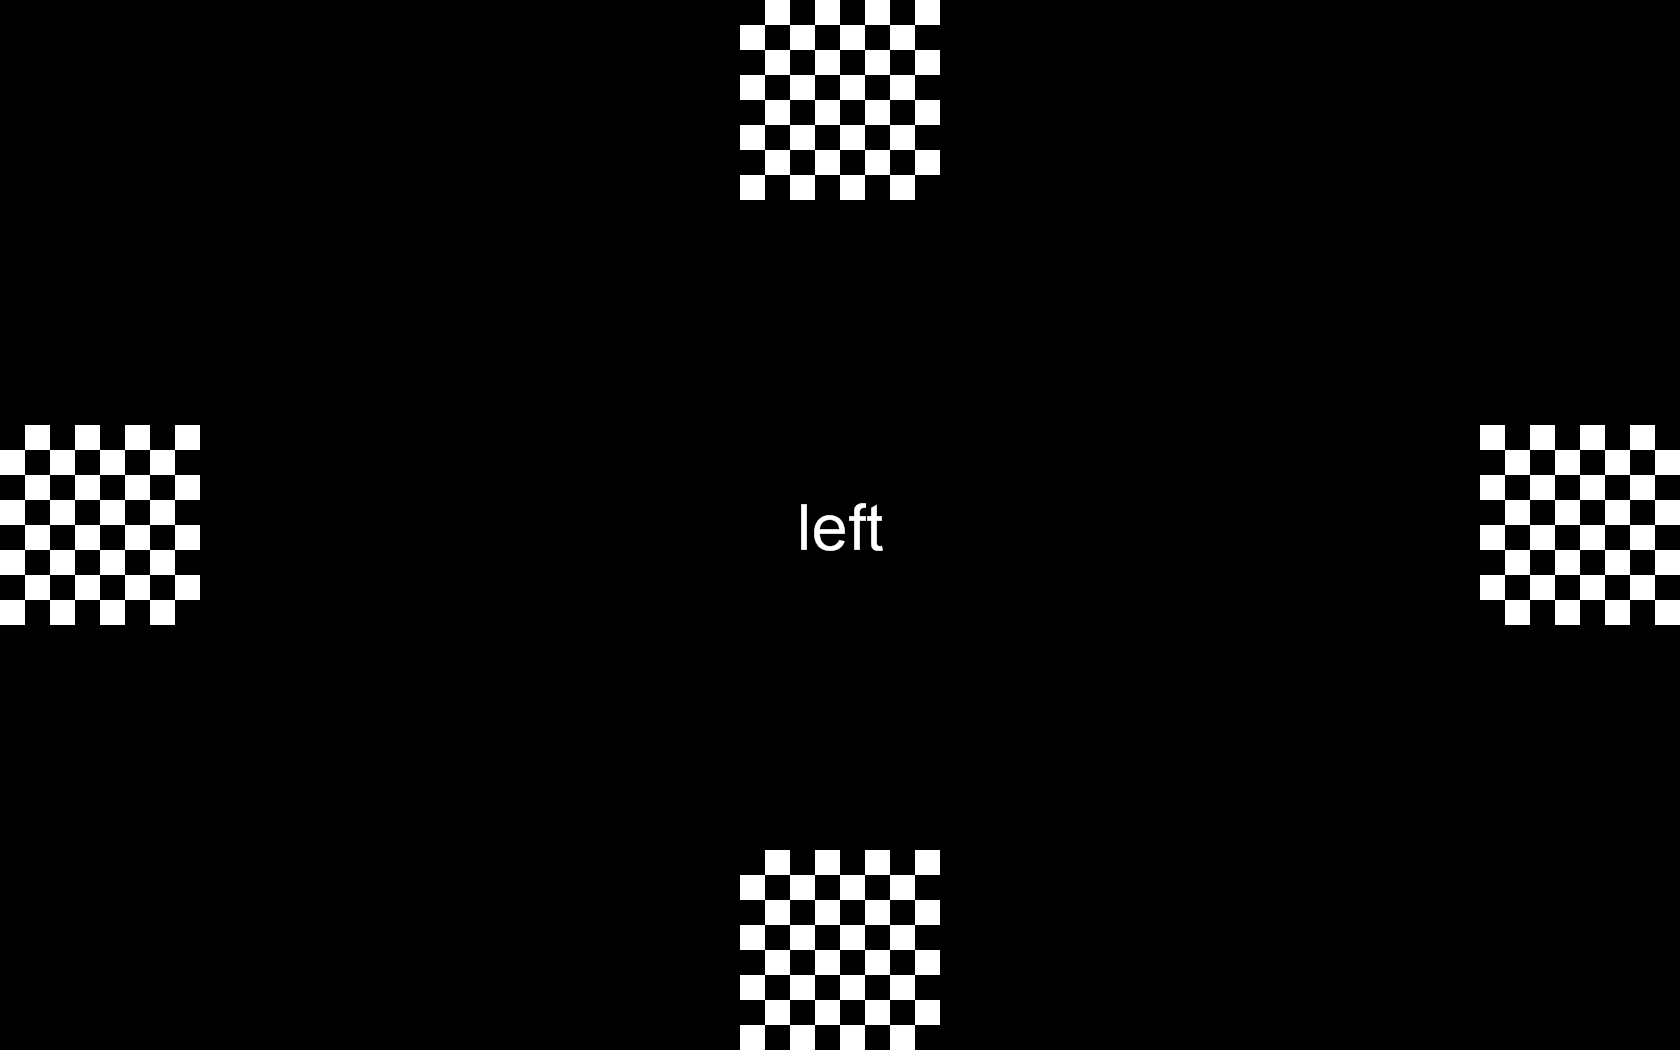
\includegraphics{images/msequence.png}}
\caption{\label{bci-pipeline-fig}  Data flow through Unlock}
\end{figure}


%\section{History}
%Unlock started, in 2011, as a Python script written by Sean Whatshisname for researching solid-state VEP %(SSVEP)[ssvepref].  In 2012, researching maximium length sequence decoding, Byron Galbraith rewrote Sean's %script into a program.  In 2013, Unlock was completely rewritten to be a programming framework.  The rewrite %was led by James Percent, with help from Byron, Nguyen Hoang Giang and other Unlock contributors. 

\section{Installation}
\subsection{Windoze}
Currently Unlock only supports Windows 7 - this was, quite painfully, required due to the nature of the users.  But  Further we believe most of the users of the system will not be programmers.  While the projects aim is to reach out to people.

 required.  Since It was originally written
by James Percent, but significantly extended by Nguyen Hoang Giang.

The windows installer was written in Go [1] (note, for Go related internet searches add the term
golang).  The reason Go was chosen is because we wanted to have a binary file that users can
download and execute without knowing the details of any of Unlock's dependencies, which there are
a few.
\subsection{Linux}
\subsection{Mac OSX}

\section{Usage}

\section{Software}
\subsection{BCI Layer}\label{bcisec}

In Section~\ref{overviewsec} we defined the signal-processing chain to be signal acquisition and reconstruction, feature extraction and decoding, and command generation.

Signal acquistion is handled by code written in C++.  The C++ layer is dynamically linked into the Python runtime using Boost Python~\cite{boostpython}.  The signal acquisition module exports a single polymorphic interface inspired by UNIX device files, and several factory methods for creating the signal acquistion infrastructure.

Unlock supports two modes of acquisition: blocking acquistion and non-blocking acquistion.  Blocking acquisition is is simply a thin wrapper around the device interface.  It will block on a I/O descriptor until a write is available.

We will discuss Unlock's application layer in detail in Section~\ref{applicationsec}.  But at this time it is important to understand at least one aspect: application layer is essentially a graphics event loop.  And as such it is sensitive to timing issues.

For this reason, Unlock supports a nonblocking acquisition mode.  This is especially important for stimulation as some of the paradigms are very senstive to timing issues.

 creates a platform independent C++ thread, using Boost Thread~\cite{boostthread}.  It transfers data using a lock-free algorithm from the acquisition thread to the Python event loop thread.

We will discuss Unlock's application layer in detail in Section~\ref{applicationsec}.  But at this time it is important to understand at least one aspect of it.  The Unlock application layer is essentially a graphics event loop, so it gets called for each screen painting.

For this reason, blocking based acquistion is only recommended for device testing purposes.  Blocking the event loop is not good.

The unlock application layer is a thin wrapper around

 supported for all devices, at this time, but it is only recommended for testing.  

Each device is exported through Boost Python and can be maniupated in Python code as if it were a native Python object.

The system supports two modes of acquisition; nonblocking-based and block-based signal acquistion.  All devices can be run in either mode.  

Data acquition systems can be opened and closed; when open the data can be aquired from the device.  The polymorhpic type of the signal acquisition base allows for many extention patterns to applied to the signal acquistion process.

To keep the layering coherent, we have co-located application level BCI code with the signal-processing chain BCI code.

\subsection{Application Layer}

The Unlock application programming layer is a model-view-controller (MVC)~\cite{mvc, mvc2} inspired framework for graphical user interface (GUI) development.  Commands flow through the BCI layer to a control layer that interprets the state changes and sends the changes to visualization module.

\subsection{Example}

\begin{thebibliography}{99}
\bibitem{lis}  Bauer, G. and Gerstenbrand, F. and Rumpl, E. Varieties of the locked-in syndrome. Journal of Neurology.  1979.
\bibitem{signalprocessing}  Sippi, C.,  Sippi, P., Computer Dictionary and Handbook. 1972. 
\bibitem{neuraleng}  He B., Gao S., Yuan H., and Wolpaw, J.  Neural Engineering, Chapter 2, Brain–Computer Interfaces.  2013.
\bibitem{abci} CELEST Capstone Project 1: Adaptive Brain-Computer Interactions.  http:\/\/celest.bu.edu/about-us/capstone-projects/adaptive-brain-computer-interactions.
\bibitem{mvc}  Reenskaug, T. A note on DynaBook requirements. Xerox PARC.  1979.
\bibitem{vep} O’Shea, R. P., Roeber, U., Bach, M. Evoked potentials: Vision.  Encyclopedia of Perception. 2010.
\bibitem{boostpython} Boost Python.  http:\/\/www.boost.org/doc/libs/1\_54\_0/libs/python/doc/.
\bibitem {npl} Unlock.  http:\/\/github.com/NeuralProsthesisLab/unlock.
\bibitem{mobilab} Gtec MOBILab.  http:\/\/www.gtec.at/Products/Hardware-and-Accessories/g.MOBIlab-Specs-Features

\end{thebibliography}

\end{document}
